\documentclass[11pt]{article}

\usepackage[margin=1in]{geometry}
\usepackage{amsmath,amssymb}
\usepackage{array}
\usepackage{booktabs}
\usepackage{enumitem}
\usepackage{hyperref}
\usepackage{listings}
\usepackage{microtype}
\usepackage{needspace}
\usepackage[T1]{fontenc}
\usepackage{lmodern}
\usepackage{xcolor}
\usepackage{tikz}
\usetikzlibrary{arrows.meta,positioning}

\hypersetup{
    colorlinks=true,
    linkcolor=blue,
    urlcolor=blue
}

\definecolor{codebg}{RGB}{247,247,247}
\definecolor{codekw}{RGB}{45,76,150}
\definecolor{codecomment}{RGB}{80,115,80}
\definecolor{codestring}{RGB}{145,70,45}
\definecolor{flowblue}{RGB}{232,240,250}

\lstdefinelanguage{Rust}{
    morekeywords={as,async,await,break,const,continue,crate,dyn,else,enum,extern,
        false,fn,for,if,impl,in,let,loop,match,mod,move,mut,pub,ref,return,
        self,Self,static,struct,super,trait,true,type,unsafe,use,where,while},
    sensitive=true,
    morecomment=[l]{//},
    morecomment=[s]{/*}{*/},
    morestring=[b]"
}

\lstset{
    language=Rust,
    basicstyle=\ttfamily\small,
    keywordstyle=\color{codekw}\bfseries,
    commentstyle=\color{codecomment}\itshape,
    stringstyle=\color{codestring},
    backgroundcolor=\color{codebg},
    frame=single,
    framerule=0.3pt,
    rulecolor=\color{black!25},
    columns=fullflexible,
    keepspaces=true,
    showstringspaces=false,
    breaklines=true,
    tabsize=4,
    xleftmargin=0.5em,
    xrightmargin=0.5em,
    aboveskip=0.8em,
    belowskip=0.8em
}

\title{\textit{cs-mail} Rust Reference Architecture}
\author{C-SQD}
\date{Draft 0.8 --- September 2026}

\usepackage{tabularx}
\newcolumntype{Y}{>{\raggedright\arraybackslash}X}
\setlength{\emergencystretch}{1.5em}

\begin{document}
\maketitle

\begin{abstract}
This architecture follows one relationship request from charge preparation to
recipient decision, then follows a forfeiture into the quarterly member program.
A pure transition computes the required state and accounting obligations. A
transaction commits them with an outbox; external providers confirm payment
effects afterward. This division gives the revised protocol a small deterministic
center while keeping delivery, payment uncertainty, and member eligibility in
explicitly bounded services.
\end{abstract}

\paragraph{Status and reading order.}
The \textit{Protocol Specification} and the normative financial-program section
of the \textit{Deployment and Migration Profile} control the rules. This document
explains their intended implementation shape. Names and fragments below are
illustrative target interfaces, not assertions that the current Rust workspace
already implements the revised model. The desktop build plan describes how to
reach that target through a simulated pilot.

\section{One Request, Three Messages, One Decision}

Alice creates a relationship request to Bob. The signed quote fixes $C+S$ and
the request's policy versions. Creation stores one payment intent; a worker
obtains capture confirmation from the external provider. Initial admission then
commits the encrypted content reference, delivery intent, common decision
deadline, and one recipient solicitation. The public-identity pair has one
nonterminal request, even if Alice submits from several devices.

Bob permits follow-ups, so Alice adds two messages. Each has distinct ciphertext,
authenticated declarations, and delivery state. Admission consumes Bob's permitted
allowance, but creates no additional charge or request-history increment and
does not move the decision deadline.

When Bob accepts, the system grants permission and records one refund obligation
for $C+S$. It closes the request and cancels expiry in the same transaction. A
worker then executes the refund. Alice may write under standing acceptance while
the provider is still confirming that refund: permission and the obligation are
already committed, although external payment completion remains pending.

\begin{figure}[ht]
\centering
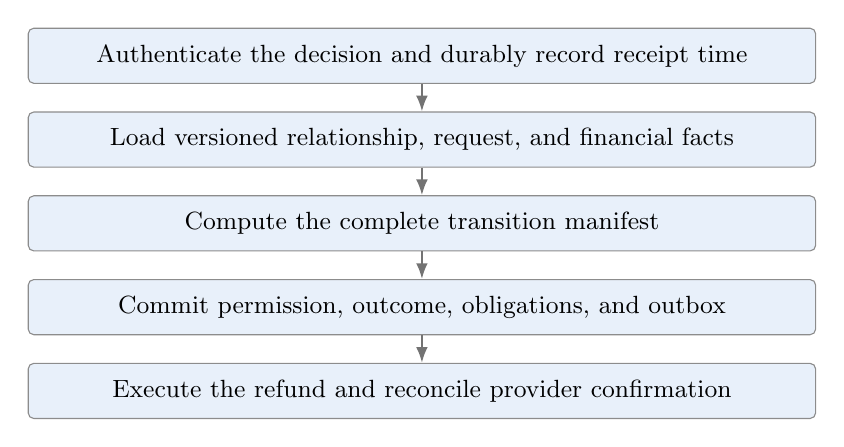
\begin{tikzpicture}[
node distance=0.35cm,
flow/.style={draw=black!45,rounded corners=2pt,fill=flowblue,
minimum width=10cm,minimum height=0.7cm,align=center,font=\small},
arrow/.style={-{Latex[length=2mm]},thick,draw=black!55}]
\node[flow] (a) {Authenticate the decision and durably record receipt time};
\node[flow,below=of a] (b) {Load versioned relationship, request, and financial facts};
\node[flow,below=of b] (c) {Compute the complete transition manifest};
\node[flow,below=of c] (d) {Commit permission, outcome, obligations, and outbox};
\node[flow,below=of d] (e) {Execute the refund and reconcile provider confirmation};
\draw[arrow] (a)--(b); \draw[arrow] (b)--(c);
\draw[arrow] (c)--(d); \draw[arrow] (d)--(e);
\end{tikzpicture}
\caption{The commit establishes the obligation; external confirmation discharges it.}
\end{figure}

\section{The Pure Transition and Its Durable Boundary}

\subsection{Authority enters as evidence}

Wire decoding first checks versions, sizes, and canonical structure. Signature
verification then binds the exact command digest to an authorized actor, key,
deployment, provider, and receipt. Finally, domain conversion checks scope and
command-specific constraints. An authenticated wrapper should have private
constructors; a public boolean claiming authentication cannot carry this meaning.

The recipient's device time is not authoritative. Ingress durably records
authenticated receipt before returning evidence to the client. That record lets a
timely acceptance beat an expiry worker even when decision processing is delayed.

\subsection{A snapshot contains the facts that can change}

For acceptance, the snapshot contains the relationship, its current request if
any, request-history context, relevant payment/refund facts, and ledger references.
It carries versions and enough completeness evidence to distinguish no current
request from a missing projection. Historical pending refunds may still exist
after a request closes; they remain separate obligations rather than additional
open relationship requests.

The pure function has a compact shape:
\begin{lstlisting}
pub fn transition(
    snapshot: &RequestSnapshot,
    command: Authorized<RequestCommand>,
    context: &TransitionContext,
) -> Result<TransitionManifest, ProtocolError>;
\end{lstlisting}
It performs no I/O and reads no implicit clock or live policy service. Time,
versions, immutable terms, and authenticated evidence are inputs. Its result
describes the complete consequence, not just a new relationship-state enum.

\Needspace{19\baselineskip}
\subsection{The manifest owns the whole consequence}

\begin{lstlisting}
pub struct TransitionManifest {
    preconditions: Preconditions,
    relationship: Option<RelationshipUpdate>,
    request: Option<RequestUpdate>,
    history: Option<RequestHistoryUpdate>,
    obligations: Vec<ObligationUpdate>,
    ledger: LedgerBatch,
    schedules: Vec<ScheduleChange>,
    events: Vec<DomainEvent>,
    effects: Vec<EffectIntent>,
}
\end{lstlisting}
Private constructors enforce agreement among these fields. An acceptance cannot
grant permission without its required request outcome and refund obligation.
A rejection cannot credit the recipient. Follow-up admission cannot introduce a
charge simply because it uses the same storage transaction machinery.

Storage verifies preconditions and commits the manifest atomically. In the
initial single-provider deployment, a serializable transaction or equivalent
lock/version discipline is a practical boundary. Application controllers do not
recompute financial consequences after the kernel returns. Transactional outbox
records make every post-commit operation recoverable.

\section{Objects That Keep Different Lifecycles Apart}

The relationship persists across requests. A request progresses from preparing
to open and then accepted, rejected, expired, or cancelled before admission.
A payment operation separately tracks external preparation, dispatch, uncertain
outcome, and confirmed facts. A refund obligation can remain unpaid after its
request is terminal. These distinctions should appear in domain types rather
than a single overloaded status field.

Use separate scoped identifiers for the relationship, request, message, payment
operation, refund obligation, forfeiture lot, quarter allocation, and member
payable. A member reference is not a public identity or a general principal
reference. Translation among domains requires explicit authority.

Money remains integer minor units with an explicit settlement unit. Checked
arithmetic rejects overflow and mixed-unit operations. Corporate rates use exact
rational or basis-point representations. Different clocks also deserve distinct
types: admission deadline, request decision deadline, message validity, maturity
cutoff, and quarter boundary do different work.

Quoted financial-policy versions remain fixed for a request. Current follow-up
policy may change and is checked at each admission under a versioned guard.
Changing notification preferences has neither authority. A future nonzero
persistence reserve needs an explicit extension; the base draft uses zero and
does not silently recycle the old reserve semantics.

\section{Payment Work Is a Recoverable Conversation}

\subsection{Create before dispatch}

Creation claims the unique nonterminal request for the directed pair and records
one authorized payment intent before calling a provider. A database uniqueness
constraint or equivalent aggregate guard prevents two devices with different
keys from dispatching two charges for the same pending relationship request.
The worker's external idempotency key derives from that committed operation,
not from a fresh network retry.

An external timeout means uncertainty. The worker queries the original operation
or repeats it under the provider's idempotency contract; it cannot assume failure
and invent a replacement. Admission waits for the profile's verified capture
evidence and durable content. The platform does not rely on an authorization
remaining open throughout the decision window.

\subsection{Cancellation can precede confirmation}

If admission timeout or sender cancellation commits first, the request stays
cancelled. The payment adapter voids an uncaptured authorization or refunds a
capture. If a capture confirmation arrives afterward, the reconciler records the
financial fact and schedules the full refund without reopening the request.
This is a normal recoverable sequence, not an exceptional database rollback.

Provider notifications are authenticated evidence. Deduplicate them by provider
event and economic operation, check amount, unit, and destination scope, and
reconcile out-of-order facts without regressing confirmed state. Both polling
and webhooks may discover the same event; neither may duplicate a refund.

\subsection{Completion is separate from obligation}

Refund and payout workers read durable obligations and execute stable operations.
Failure leaves an obligation pending or under review. Success records reconciled
confirmation and the corresponding ledger effect. A chargeback or adjudicated
correction appends a separately authorized batch. It does not overwrite a
recipient decision or confiscate a finalized member allocation.

The ledger therefore projects request charges, refunds due and completed,
pending forfeitures, corporate revenue, restricted member funds, and payables.
It does not expose a user wallet. A refund or payable cannot be applied as
available funds for another request.

\section{From a Rejection to a Quarterly Allocation}

Bob's rejection terminally records the request outcome, processing revenue $C$,
and a pending forfeiture lot for $S$. The lot retains the request's quoted rate
version. No immediate recipient payout is created, and no distribution worker
can treat that new lot as mature merely because a quarter ended.

Maturity evaluation is a separate deterministic decision over verified financial
facts and approved policy. It excludes refunds, unresolved disputes, and required
reserves. At cutoff, a funding manifest identifies the exact newly eligible lots.
A membership manifest independently fixes the qualifying active members. The
financial profile defines the once-only corporate calculation, equal allocation,
and integer remainder; the architecture reuses those formulas rather than
maintaining another interpretation.

Quarter finalization should produce a reproducible batch with input digests,
policy versions, assessment marks, corporate amount, member contribution,
individual payables, and unallocated carryforward. A large population can be
prepared in bounded chunks, but readers must not see a partially finalized
quarter. A commit marker or equivalent atomic manifest makes the prepared result
visible once and prevents a retry from assessing the same lots again.

Payout execution then follows the same obligation/outbox pattern as refunds.
Failed payments and below-threshold amounts remain assigned to their members.
They are not included in the following quarter's unallocated pool. Corrections
to eligibility or external losses require authorized new entries with a funding
source and audit cause; recomputing the old snapshot in place is not recovery.

\section{Admission, Scheduling, and Concurrency}

All delivery paths observe blocking under the directed-pair transaction boundary.
Standing acceptance and valid lanes authorize delivery without a request charge.
An authenticated follow-up additionally identifies an open request and consumes
the recipient's current allowance. Only eligible new-request creation may start
a new payment operation, and it requires explicit sender authorization.

Follow-up policy updates, request closure, and delivery admission serialize.
Content and a retryable delivery effect must be durable before admission commits.
Message validity is checked independently of the request's common deadline.
Lanes retain their signed scope and hard validity limits; granting or revoking a
lane does not settle a request or create member activity.

Scheduled work includes preparing-request timeout, request expiry, payment
reconciliation, maturity review, quarter preparation, payout retry, and retention.
Each job carries a target, earliest execution time, version/evidence preconditions,
and stable operation identity. Leased workers submit commands against current
state. They do not assume that a row remains unchanged because a job was queued.

Principal-scoped new-request history needs its own concurrency guard shared by
aliases. It advances only at initial admission. A follow-up, cancelled preparation,
or key rotation cannot bypass that distinction. Late acceptance changes future
permission while old expiry processing preserves that permission and materializes
only the old request's financial obligation.

\section{Responsibility Boundaries in the Workspace}

The existing separation of primitives, security, ledger, protocol, application,
storage, and adapters remains useful. The semantic revision changes their
contracts before product layers rely on them. Primitives define constrained money,
time, versions, and scoped references. Security produces verified evidence.
The request kernel computes outcomes; the ledger proves accounting conservation.
Application and storage apply complete manifests. Payment adapters translate
provider evidence and execute operations without inventing settlement rules.

The member program is a separate domain module for eligibility, maturity, and
quarter finalization. It may reuse ledger, scheduling, and outbox contracts but
should not be embedded in message controllers. A separate crate is warranted
only when it supplies a stable independently useful boundary. A separate process
is warranted by credentials, data access, failure isolation, or scale; a crate
alone does not enforce privacy.

Content and wire modules retain authenticated encryption and declaration binding.
Capability admission remains a permission path beside financial transitions.
The client owns presentation and endpoint secrets; it consumes signed outcomes
instead of reconstructing financial rules. API, wire, event, protocol, database,
and financial-policy versions remain distinct.

\section{Privacy Extends to the Member Program}

No routine component needs the entire story. The identity service knows control
and recovery evidence. The relationship service sees scoped permission and request
state. Content storage sees ciphertext. The ledger sees scoped financial causes
and amounts. Membership verification sees the evidence needed to establish one
qualifying member, while the allocation engine can consume a minimal eligibility
assertion. Telemetry receives short-lived, rotated references.

Use separate access roles, keys, and credentials, including for financial and
membership records that must outlive ordinary delivery data. Public identities
and private principals must not become universal ledger or telemetry join keys.
Native content is encrypted at endpoints; a payment or membership check does
not authorize provider decryption. Authenticated purpose and origin remain
accountable declarations, not proof of plaintext truth.

Eligibility activity should record only the minimal facts required by policy.
Background synchronization and inbound lane traffic are not substitutes for
intentional use. The payment provider receives required transaction references
and amounts, not message content or the user's unrelated relationships.

Retention classes define purpose, key scope, operational lifetime, dispute or
required retention, and deletion method. A settled request can lose unnecessary
message linkage while an unpaid refund or member payable retains enough evidence
for payment and audit. Continuing permission does not justify retaining its
formation history forever. Cryptographic erasure must cover wrapped keys,
replicas, backups, logs, and derived indexes; separately retained records must
not be described as erased or two-party-only archives.

Logs and errors use safe event types and redacted identifiers. They must contain
no plaintext, secrets, complete financial snapshots, or private identity evidence.
Pairwise scoping reduces direct linkage but does not eliminate timing or amount
correlation, so retention and access discipline remain necessary.

\section{Migration and Evidence of Correctness}

First establish a new protocol/version baseline and document how any existing
quotes, requests, and obligations would be treated. Do not reinterpret stored
per-message bonds by renaming their fields. Old financial expectations need
explicit replacement vectors, while applicable authentication, privacy, ordering,
and conservation guarantees remain protected.

The first story test uses one charged request and three permitted messages.
Acceptance creates one refund obligation, and provider confirmation completes it
once. Variants reject into pending forfeiture, expire into a collateral refund,
disable follow-ups, and race policy changes with admission. Other tests exercise
two-device creation, alias history, cancellation followed by late capture,
duplicate/out-of-order notifications, and unknown commit recovery.

Financial-program tests reproduce a quarter from fixed input manifests, exclude
refundable and immature funds, assess each eligible lot once, preserve quoted
rate cohorts, and allocate equal integer shares. Include zero members, small
amounts, unallocated remainder, below-threshold payables, failed payments, and
quarter retries after a crash. A later quarter must not assess old member funds
or redistribute already assigned obligations.

Property and concurrency tests check conservation, finality, uniqueness, scope,
and recovery at durable boundaries. Privacy tests exercise cross-domain credential
denial, captured-log redaction, and deletion through backup restoration. Fuzz
canonical decoding, signatures, and content bindings.

Independent-provider federation follows only after a financial agreement assigns
pool governance, membership uniqueness, refund and payout obligations, clearing,
and losses. The local manifest remains useful as a reference outcome, but the
old direct-recipient clearing model is not carried forward automatically.

\end{document}
